\chapter{The ATLAS Detector} \label{chapter-atlas}

ATLAS is a system of particle detectors built to
measure collisions of both proton-proton and heavy ion collisions
generated by the LHC. \cite{atlas-detector-2008} The entire detector
is $44~m$ long and $25~m$ in diameter. It consists of an inner
detector subsystem for charged particle tracking and electron
identification, both electromagnetic and hadronic calorimeters, and a
muon spectrometer.

\section{Coordinates}
The coordinate system used in this document is the standard ATLAS
coordinate system, which is defined in this section. For both Cartesian and
polar coordinates, the origin is defined as the nominal interaction
point. The z-axis points down the beamline. The x-y plane is
perpendicular to the beamline. The positive y-direction points up, and
the positive x-direction points towads the center of the LHC ring. The
positive z-direction therefore points counterclockwise along the LHC,
when view from above, as required by a right-handed coordinate system.

For cylindrical coordinates, the z-axis is defined the same way as for
Cartesian coordinates. The azimuthal angle $\phi$ is the angle
from the positive x-axis, while the polar angle $\theta$ is the angle
from the beamline.

A more convenient measure of angle from the beamline is the
\textit{rapidity}, because rapidity differences are invariant under Lorentz boosts in the
z-direction. The rapidity is defined as:
\begin{equation}
y = \frac{1}{2}\ln\frac{E+p_z}{E-p_z}
\end{equation}

Another frequently used quantity is the
\textit{pseudorapidity}, which is defined as:
\begin{equation}
\eta = -\ln\frac{\theta}{2}
\end{equation}

Pseudorapidity differences are also invariant with respect to
longitudinal Lorentz boosts. In the limit where $p_T << m$, rapidity and
pseudorapidity are equal.

Pseudorapidity ranges from $\eta=0$, which is perpendicular to the
beamline, up to $\eta=\inf$, which is parallel to the beamline.

Finally, a distance measure in $\eta-\phi$ space is often used. This
distance, $\Delta R$ is defined as:

\begin{equation}
\Delta R = \sqrt{\Delta\eta^2+\Delta\phi^2}
\end{equation}

\section{Magnet System}

\section{Inner Detector}

The inner detector consists of silicon pixel detectors, silicon strip
detectors, and transition radiation trackers. It covers a region from
$R = 33~mm$ to $R = 1082~mm$ and $|\eta| = 0$ to $|\eta| = 2.5$. The entire inner
detector is immersed in a $2~T$ magnetic field, generated by a
solenoid coil which surrounds it.\cite{atlas-detector-2008} The layout of inner detector
subsystems is shown in figure \ref{fig:inner_detector_quarter}.

\begin{figure}[h]
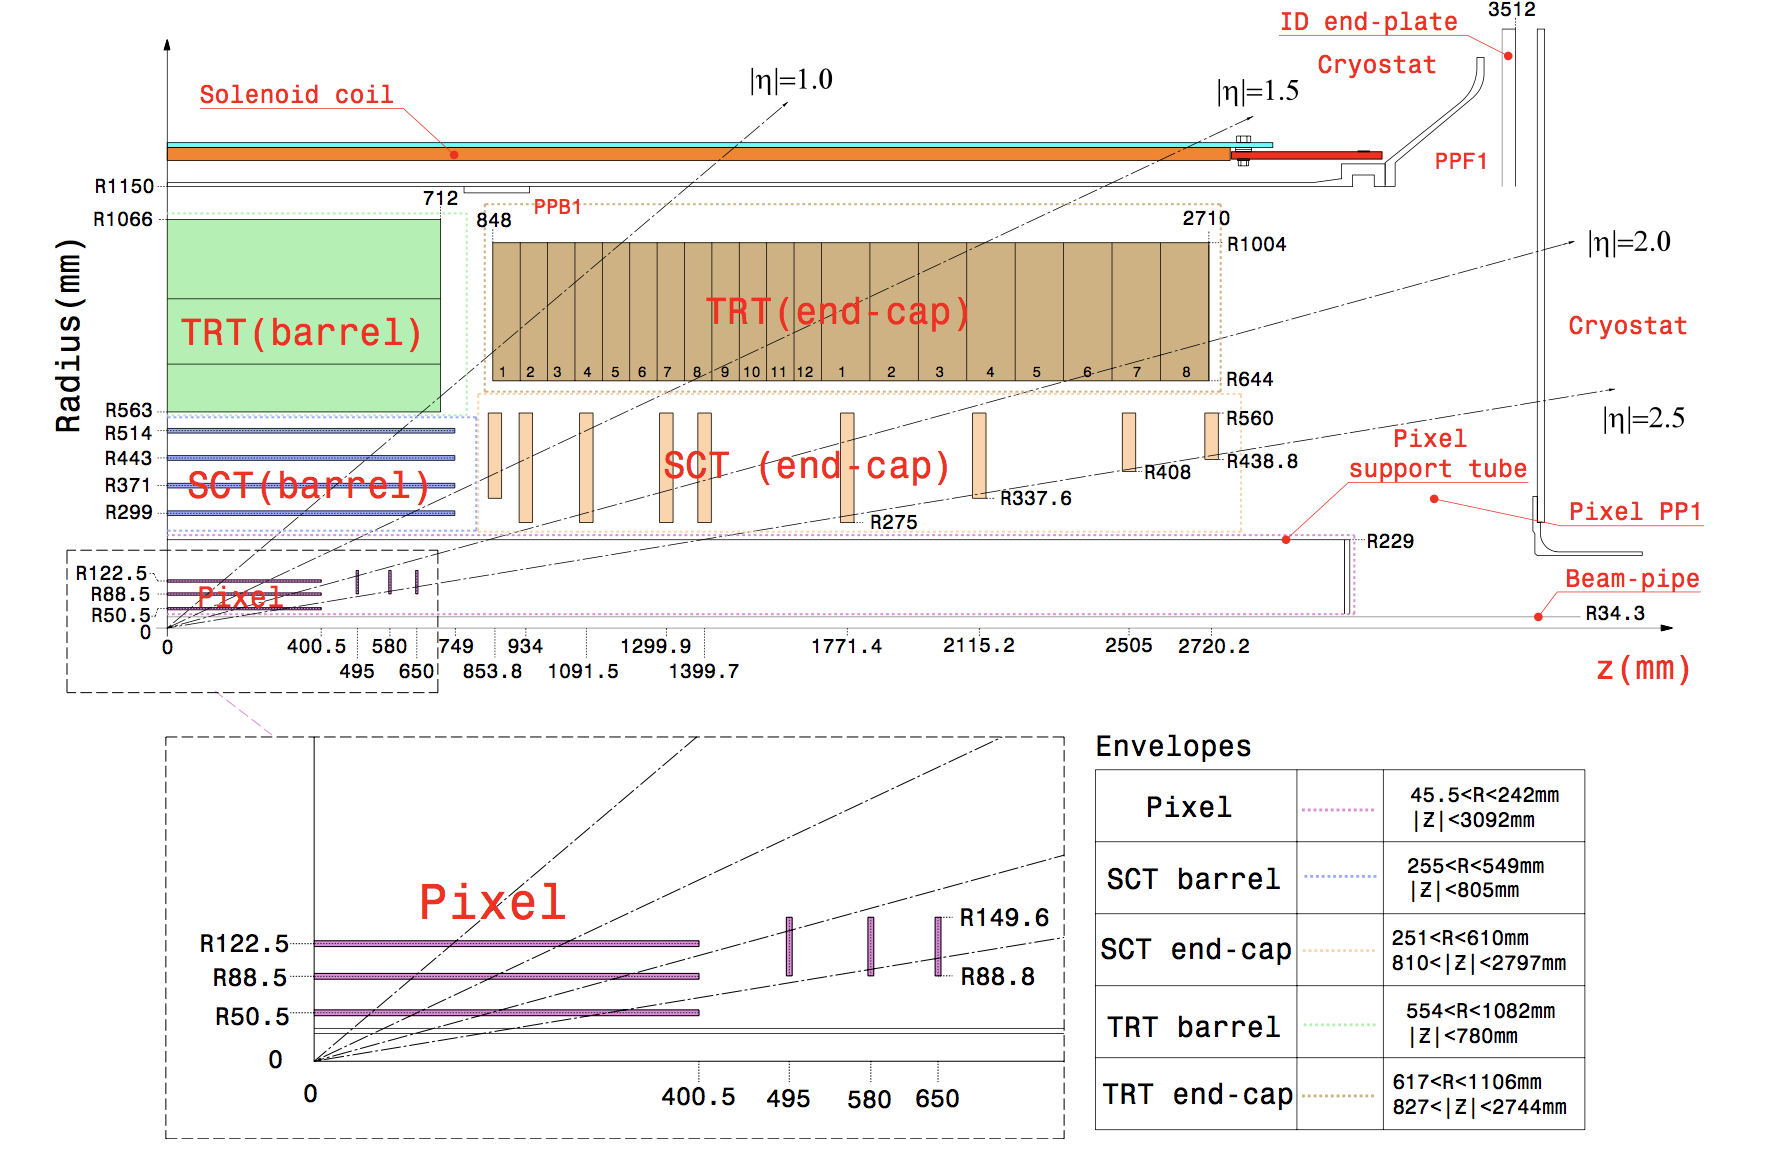
\includegraphics[width=\textwidth]{inner_detector_quarter}
\caption{A quarter-section plan showing the layout of inner detector
  susbystems and their dimensions. Not shown is the innermost layer of
the pixel detector, the IBL, which was installed in May 2014.}
\label{fig:inner_detector_quarter}
\end{figure}

\subsection{Pixel Detector}

The innermost layer of ATLAS is the pixel detector system. It consists
of 1744 solid-state pixel sensors, arranged into a barrel region and two endcap
regions. In total, there are 80.4 million pixel readout channels. \cite{atlas-detector-2008}

\subsubsection{Layout}
The barrel region consists of four
concentric cylindrical layers, coaxial with the beamline. The two endcap regions are each made up
of three disks, arranged perpendicular to the beamline.

The pixel barrel envelope covers a region
from $z = 0$ to $|z|  = 400.5~mm$. The four layers are located at
increasing distances from the beamline, at $R = 33~mm, 50.5~mm,
88.5~mm, 122.5~mm$.

The six endcap disks are located at $|z| = 495~mm, 580~mm, 650~mm$
and cover the region $88.8~mm < R < 149.6~mm$. \cite{atlas-detector-2008}

Figure ~\ref{fig:inner_detector_quarter} shows a quarter-section of
the entire inner detector, as well as a detailed view of the pixel
subsystem, not including the Insertable B Layer (IBL), which was
installed in 2014.

\subsubsection{Sensors}
The ATLAS pixel sensors are solid-state silicon detectors. The basic operating
principle of a solid-state detector is that charged particles passing
through the material generate electron-hole pairs, which are
accelerated towards opposite ends of the material via an electric
field. This generates a current, which can be measured by
charge-sensitive sensors at the edge of the material.\cite{spieler-2005}

In a silicon detector, the active material is a pn junction, operated
with a reverse bias voltage, until fully depleted. This reduces the thermal noise
from free charge carriers to a low enough level that electron-hole pairs from
signal particles can be detected.\cite{spieler-2005}

In ATLAS, the pixel sensors consist of an n-type bulk, with $p^+$
implants on the back side and $n^+$ implants on the front side. Before
irradiation, the active pn junction region exists between the n-type bulk and $p^+$-
implanted side. Irradiation leads to the reduction in the effective
doping concentration, until the bulk material undergoes type
inversion. After type inversion, the active pn junction region
switches to the $n^+$-doped side.\cite{pixels-2008} This process is illustrated in
Figure ~\ref{fig:pixel_type_inversion}.

This $n^+$-in-$n$ design allows the sensors to continue to operate
both before and after large doses of radiation.

Each pixel tile has 47232 pixels, layed out in a grid of 144 columns
by 328 rows. Some of the pixels are grouped to common read-out
channels, resulting in 46080 read-out channels. This grouping is done
so that an equal number of read-out channels can be connected to each
of the 16 front-end read-out chips.

In 128 of the columns, each pixel implant is $382.5\times30~\mu m^2$,
with pitch (center-to-center distance) of  $400\times50~\mu m^2$. In
the remaining 16 columns, the pixel sizes are $582.5\times30~\mu m^2$,
with a pitch of  $600\times50~\mu m^2$.\cite{pixels-2008}

\begin{figure}[h]
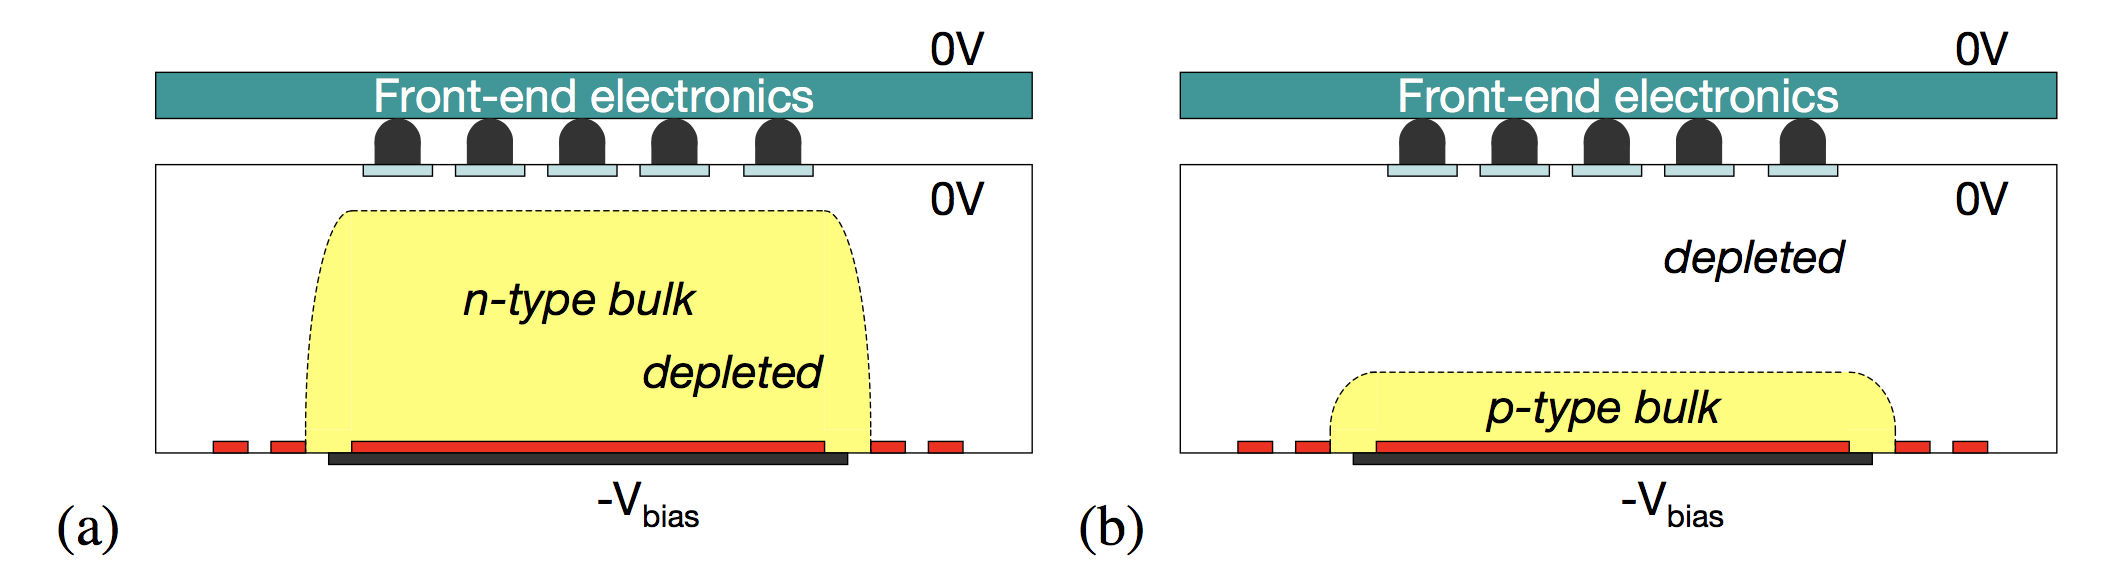
\includegraphics[width=\textwidth]{pixel_type_inversion}
\caption{Graphic illustrating how $n^+$-in-$n$ pixel sensors continue
  to operate after the type inversion that results from
  irradiation. In (a), the unirradiated state, the bulk is n-type, and
the depletion zone occurs between the $p^+$-doped back side. After
type inversion, in (b), the depletion zone occurs between the now
p-type bulk and the $n^+$-doped front side.\cite{pixels-2008}}
\label{fig:pixel_type_inversion}
\end{figure}

\subsubsection{The IBL}
A major upgrade that occurred during the long shutdown in 2014 was to
install the Insertable B-Layer (IBL) to the pixel detector. The IBL became
the fourth and innermost layer of the pixel detector. The IBL provides
several key improvements to the tracking system, which will allow the
pixel detector to maintain good performance even in the
higher-luminosity environment that will be present in the High
Luminosity LHC (HL-LHC).\cite{ibl-tdr} The IBL does this by
improving tracking robustness against module failures, adding
measurement redundancy to mitigate the effects of pileup, and
adding an additional measurement closer to the interaction
point. \cite{ibl-tdr}

As part of the IBL insertion project, the original beam pipe was
removed, and replaced with a smaller-radius beampipe. Precision
tooling and methods for insertion were developed and practiced for two
years before the procedure was finally carried out. The tolerances
were extremely tight, with only a $0.2~mm$ gap between the IBL and
inner supporting tube.\cite{ibl-website}. An image of the IBL being inserted can be seen in
~\ref{fig:ibl_insertion}

\begin{figure}[h]
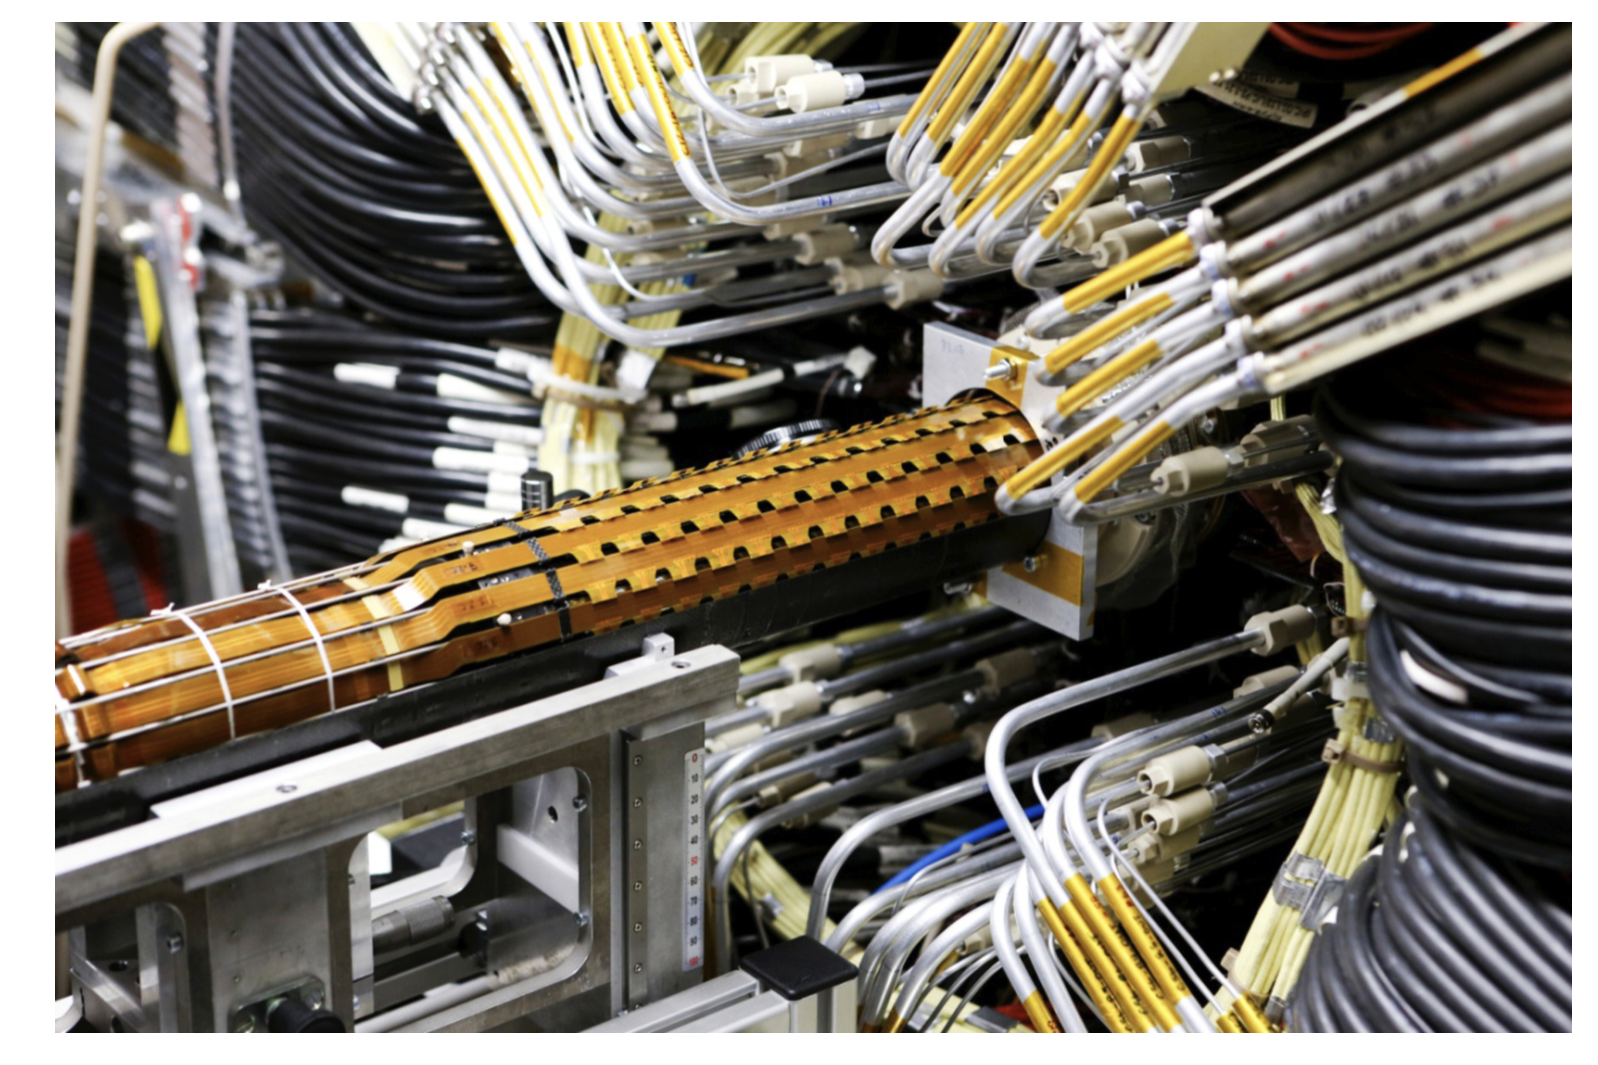
\includegraphics[width=\textwidth]{ibl_insertion}
\caption{The IBL as it was inserted into the pixel detector}
\label{fig:ibl_insertion}
\cite{ibl-website}
\end{figure}

\subsection{Silcon Strip Tracker}

The silicon strip tracker (SCT) is segmented into a barrel region and
two endcap regions. 

\subsubsection{Layout}

\subsubsection{Modules}

\subsection{Transition Radiation Tracker}

\subsubsection{Layout}
\subsubsection{Modules}

\section{Calorimeters}
\subsection{Electromagnetic Calorimeters}
\subsection{Hadronic Calorimeters}
\section{Muon Spectrometer}
\section{Trigger and Data Acquisition}